\section{Research}

\subsection{June 28}
\begin{lemma}
    For $\alpha_1, \alpha_2\in(0,1), \alpha_1>\alpha_2$, $V\in G(1,2)$, a cube $Q\in \rr^2$ with side length $2^{-|k|}$, and a cube $R$ with the same side length as $Q$ satisfies
    \begin{equation}\label{eq:condition-GDBC-2}
        R\in C_\calB^{1,1}(Q, V, \alpha_1) \quad\text{ and }\quad R\in  C_\calB^{1,2}(Q, V, \alpha_2)
    \end{equation}
    And if $s, t\in \nn$ are coefficients of the dilation cube and $d=|\centerof Q-\centerof R|$ such that 
    \begin{equation}\label{eq:tRcover2sQ-cond}
        d+\frac{\sqrt{2}}{2}\leq s \leq \sqrt{2}d-1 \quad\text{ and }\quad t \geq 2d + 2\sqrt{2}s
    \end{equation} 
    Then 
    \begin{equation}\label{eq:tRcover2sQ-conclusion}
        sQ\cap R = \emptyset \quad\text{ and }\quad R\subset 2sQ\subset tR
    \end{equation}
\end{lemma}
\begin{proof}
    Note that by Lemma \ref{lemma:Guarantee-Distance-containQ-Between-2alpha}, to satisfy (\ref{eq:condition-GDBC-2}),   
    \begin{equation*}
        \begin{split}
            d \geq \left|\frac{2 - 2\alpha_2}{\alpha_1-\alpha_2}-\sqrt{2}\right|
        \end{split}
    \end{equation*}
    For any $q\in sQ, q^\prime\in R$, by (\ref{eq:tRcover2sQ-cond}), 
    \begin{subequations}
        \label{s}
        \begin{align}
            |\centerof sQ - q| &\leq \frac{\sqrt{2}s}{2}\side Q \leq \left|\left( d-\frac{\sqrt{2}}{2}\right )\right|\side Q  \notag \\
            &\leq ||\centerof Q-\centerof R|-\frac{\sqrt{2}}{2}\side R| \notag \\
            &\leq ||\centerof Q-\centerof R| - |\centerof R - q^\prime|| \notag \\
            &\leq |\centerof Q-q^\prime| \label{eq:qprimeQfaraway} \\ 
            &\leq \left (d + \frac{\sqrt{2}}{2}\right)\side Q \notag \\
            &\leq s\cdot \side Q \notag \\
            &= \frac{1}{2}\side 2sQ\label{eq:Rinside2sQ}
        \end{align}
    \end{subequations}
    Equation (\ref{eq:qprimeQfaraway}) implies that $sQ\subset B(\centerof Q, \frac{\sqrt{2}}{2}\side 2sQ)$, $q^\prime \notin B(\centerof Q, \frac{\sqrt{2}}{2}\side 2sQ)$ $\Rightarrow sQ\cap R = \emptyset$. Besides, (\ref{eq:qprimeQfaraway}) to (\ref{eq:Rinside2sQ}) implies that $R\subset B(\centerof Q, \frac{1}{2}\side 2sQ)\subset 2sQ$. For the choice of t, assume $\forall q^{\prime\prime}\in 2sQ$, then
    \begin{equation*}
        |\centerof R - q^{\prime\prime}|\leq (d+\sqrt{2}s)\side Q \leq \frac{t}{2}\side R
    \end{equation*}
    which implies that $2sQ \subset B(\centerof R, \frac{1}{2}\side tR)\subset tR$. Then, (\ref{eq:tRcover2sQ-conclusion}) is concluded. 
\end{proof}


\begin{figure}[H]
    \centering
    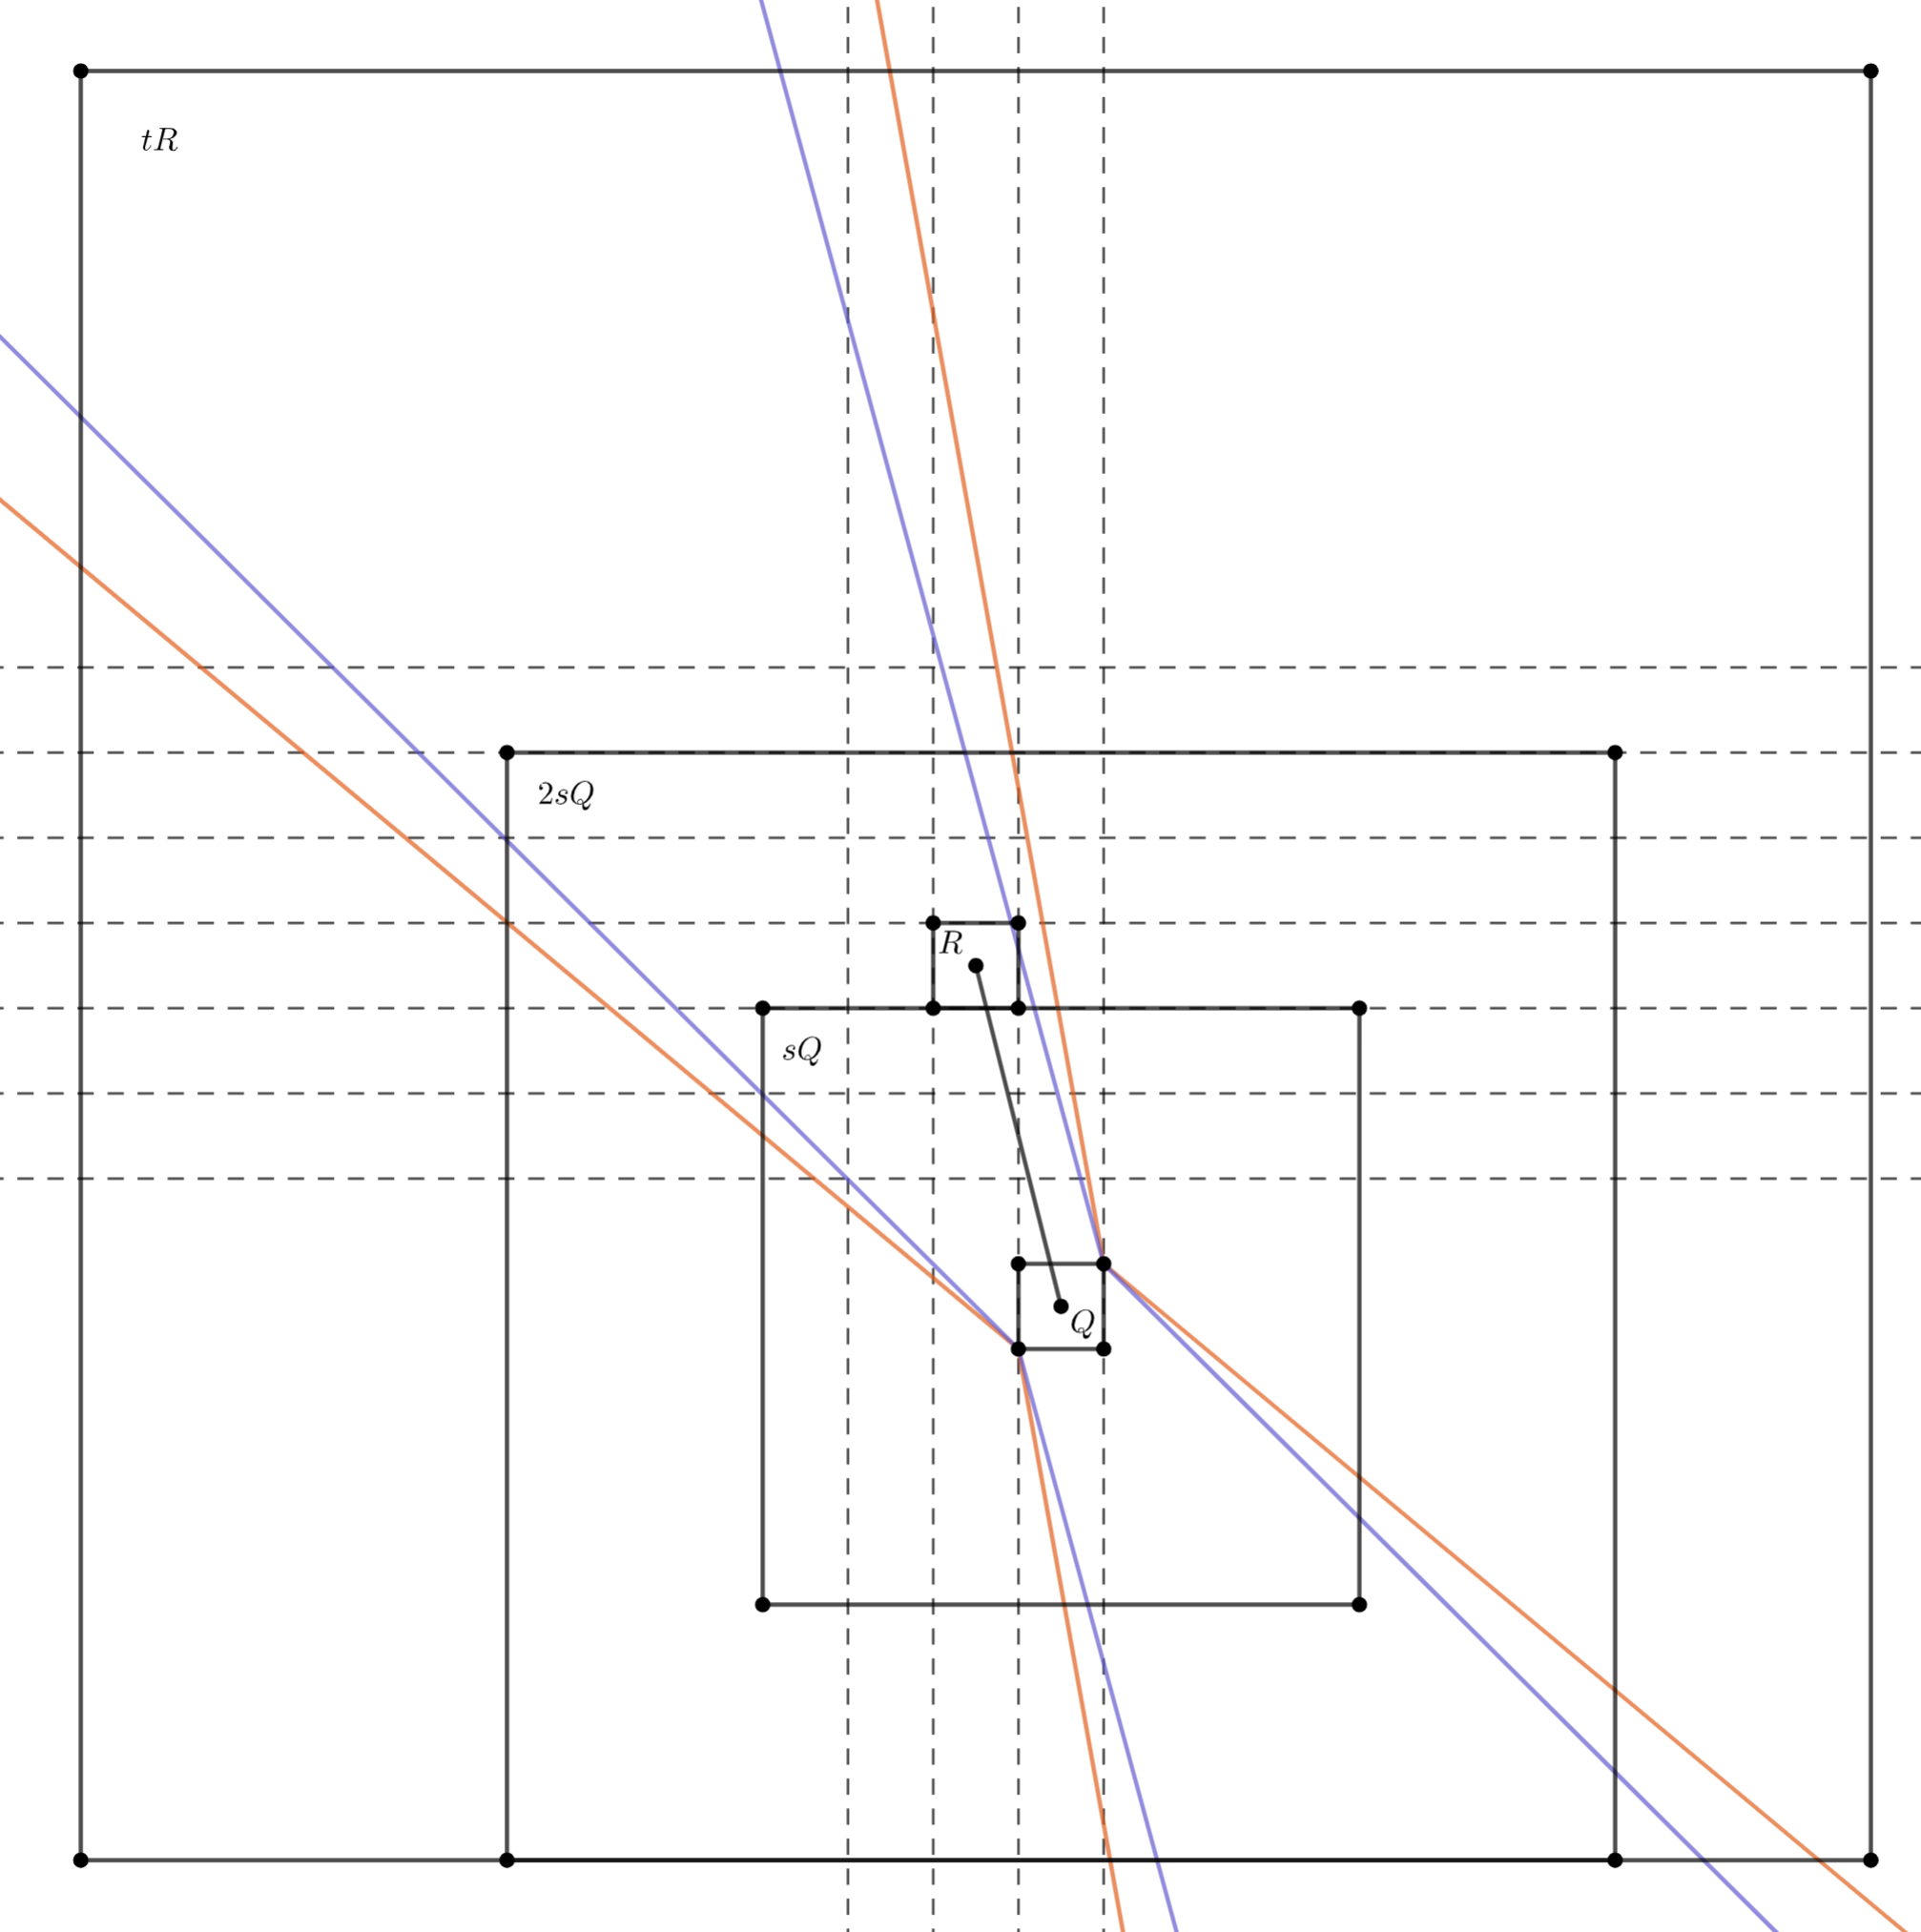
\includegraphics[width=.8\textwidth]{images/tRcover2sQ.png}
    \caption{An example in the proof on $\rr^2$}
\end{figure}


\newpage
\subsection{June 25-27 Modified Lemmas and New Lemmas}
\begin{lemma}
    If for $\mu$-a.e. $x\in \rr^2, \mu(B(x, 2r))\leq K\mu(B(x,r)), K\in\rr^+$, then
    $$\mu(5Q)\leq K^4 \mu(3Q)$$ where $Q$ is the dyadic cube, and $5Q$, $3Q$ are dilation cubes such that $\side 3Q = 3\side Q$, $\side 5Q = 5\side Q$, and $\centerof 5Q = \centerof 3Q = \centerof Q$.
\end{lemma}
\begin{proof} By the half open definition of the dyatic cube, for $\mu$-a.e. $x\in \rr^2$, $x$ must in only one cube $Q$. Let $r = \side Q /2$(in $\rr^2$). We first claim that $5Q\subset B(x, 16r)$ and $B(x, r)\subset 3Q$. As for any $q\in 5Q$, $|\centerof Q -x|\leq \sqrt{2}\cdot\side Q /2$ and $|\centerof 5Q -q|\leq \sqrt{2}\cdot\side 5Q /2 = 5\sqrt{2}\cdot \side Q/2$, 
    \begin{equation*}
        |x-q| = |x-\centerof Q + \centerof 5Q-q | \leq 3\sqrt{2}\cdot \side Q < \frac{16\side Q}{2} = 16r
    \end{equation*}
Then $q\in B(x, 16r)$ and thus $5Q\subset B(x, 16r)$. Similarly, for any $q^\prime\in B(x, r)$, 
\begin{equation*}
    |\centerof 3Q - q^\prime| = |\centerof Q - x + x-q^\prime| \leq \frac{\sqrt{2}\cdot\side Q}{2} + r < \frac{3\side Q}{2} = \frac{1}{2}\side 3Q
\end{equation*}
Then $q^\prime\in 3Q$ and thus $B(x, r)\subset 3Q$. Therefore, by the containments and the doubling measure condition, 
    \begin{equation}
        \mu(5Q) \leq \mu(B(x, 16r)) \leq K^4\mu(B(x,r))\leq K^4\mu(3Q)
    \end{equation}
\end{proof}

\begin{figure}[H]
    \centering
    \includegraphics[width=.56\textwidth]{images/doubleMucube.png}
    \caption{An example of containment in the proof on $\rr^2$}
\end{figure}


\begin{lemma}\label{lemma:CBQ2=0-carried}
    Let $\mu$ be a Radon measure on $\rr^n$, $V$ be an $m$-dimensional linear plane in $\rr^n$, $\alpha\in(0,1)$. Suppose $E\subset \rr^n$ such that for $\mu$-a.e. $x\in E$, and for every dyadic cube $Q$ containing $y$, 
    \begin{equation}\label{eq:muB2Q=0}
        \mu(C_\calB^2(Q, V, \alpha)) = 0
    \end{equation}
    Then $\mu$ is carried by $m$-Lipschitz graphs(i.e. $E$ is contained $\mu$-a.e. in an m-Lipschitz graph.)
\end{lemma}

\begin{proof}
    we first claim that if every dyadic cube $Q_k\ni x$ in the form of (\ref{eq:dyadiccube}) with side length $2^{-|k|}$ satisfies (\ref{eq:muB2Q=0}), 
    then
    \begin{equation}\label{eq:CBx=0}
        \mu(C_\calB(x, V, \alpha)) = 0
    \end{equation}
    Fix arbitrary $q_1\in Q_k$, if arbitrary $p\in C_\calB(q_1, V, \alpha)$, we have $\dist(p-q_1, V) > \alpha|p-q_1|$ by definition of bad cones. Now choose $\epsilon_p>0$ that satisfies $\dist(p-q_1, V) \geq \alpha (|p-q_1|+\epsilon_p)$. Then, for another point $q_2$ in $Q_k\ni q_1$, we have $|q_1-q_2|\leq \sqrt{n}\cdot 2^{-|k|}$. Hence, there exists a large enough $|k_p|$ such that $|q_1-q_2|<\alpha\epsilon_p/2<\epsilon_p/2$. Then,
    \begin{equation*}
        \begin{aligned} 
            \dist\left(p-q_2, V\right) & \geq \dist(p-q_1, V)-\left|q_1-q_2\right| \\ 
            & \geq \alpha(|p-q_1|+\epsilon_p)-\alpha(\epsilon_p / 2) \\ 
            & =\alpha(|p-q_1|+\epsilon_p / 2) \\ 
            & >\alpha\left(|p-q_1|+\left|q_2-q_1\right|\right) \\ 
            & \geq \alpha\left(\left|p-q_2\right|\right) 
    \end{aligned}
    \end{equation*}
    It follows that $p\in C_{\calB}^2(q_2, V, \alpha)$ and thus $p\in \bigcap_{q_i\in Q}C_\calB(q_i, V, \alpha) = C_\calB^2(Q_{k_p}, V, \alpha)$. Accordingly, for any $x\in E$, if any $p\in C_\calB(x, V, \alpha)$, then $p\in C_\calB(Q_k, V, \alpha)$, $x\in Q_k$ for some $|k|$, which implies
    \begin{equation}\label{eq:CBx-subset-UCBQ}
        p\in \bigcup_{|k|=1}^\infty C_\calB^2(Q_k, V, \alpha)\Rightarrow C_\calB(x, V, \alpha)\subset \bigcup_{|k|=1}^\infty \left\{C_\calB^2(Q_k, V, \alpha): Q_k\ni x\right\}
    \end{equation}
    Combining (\ref{eq:muB2Q=0}) and (\ref{eq:CBx-subset-UCBQ}), for $\mu$-a.e. $x\in E$,
    \begin{equation*}
        \mu(C_\calB(x, V, \alpha)) \leq \mu\left(\bigcup_{k=1}^\infty  \left\{C_\calB^2(Q_k, V, \alpha): Q_k\ni x \right \}\right) = 0
    \end{equation*}
    Therefore, (\ref{eq:CBx=0}) holds immediately and after applying corollary \ref{LisaCoro7.1}, we obtain the desired result.
\end{proof}

\newpage
\subsection{June 23-24 Lemma of Guarantee Distance Between Cubes}

\begin{lemma}\label{lemma:Guarantee-Distance-containQ-Between-2alpha}
    For $\alpha_1, \alpha_2\in(0,1), \alpha_1>\alpha_2$, a $m$-plane $V$ in $\rr^n$, a cube $Q$ with side length $2^{-|k|}$, and a cube $R$ with the same side length as $Q$, the distance bewteen the center of $R$ and the center of $Q$ has to satisfy
    \begin{equation*}
        |\centerof Q-\centerof R|\geq \left|\frac{2\sqrt{n} - 2\alpha_2}{\alpha_1-\alpha_2}-\sqrt{n}\right|\cdot 2^{-|k|}
    \end{equation*}
    to guarantee
    \begin{equation}\label{eq:condition-GDBC}
        R\in C_\calB^{1,1}(Q, V, \alpha_1) \quad\text{and}\quad R\in  C_\calB^{1,2}(Q, V, \alpha_2)
    \end{equation}
\end{lemma}
\begin{proof} 
    By assumption, there are some $x\in R\cap C_\calB^{1, 1}$ such that there exists $q\in Q$ and $x\in C_\calB(q, V, \alpha_1)$. Then $\dist(x-q, V) > \alpha_1|x-q|$. Now assume that $|x-q| = s\cdot 2^{-|k|}$. Then to satisfy (\ref{eq:condition-GDBC}), for any $y\in R$, there exists $q^\prime\in Q$ such that $y\in C_\calB(q^\prime, V, \alpha)$. Now we have $|x-y|\leq \sqrt{n}2^{-|k|}$, $|q-q^\prime|\leq \sqrt{n}2^{-|k|}$. Since $ |x-y| \geq|\dist (y-q^\prime, V)-\dist(x-q, V)| - |q-q^\prime|$, no matter $\dist (y-q^\prime, V)\lesseqgtr\dist(x-q, V)$,
    \begin{equation*}
        \begin{split}
            \dist(y-q^\prime, V) &\geq \dist(x-q, V)-|q-q^\prime|-|x-y| \\
            &> \alpha_1|x-q| - \sqrt{n}2^{-|k|+1}\\
            &= \alpha_1 s 2^{-|k|} - \sqrt{n}2^{-|k|+1}
        \end{split}
    \end{equation*}
    To guarantee that $\dist(y-q^\prime, V) > \alpha_2|y-q^\prime|$, we let $\alpha_1 s 2^{-|k|} - \sqrt{n}2^{-|k|+1} \geq  \alpha_2|y-q^\prime|$ then the assumption holds. Equivalently,
    \begin{equation*}
        \begin{split}
            \alpha_1 s 2^{-|k|} - \sqrt{n}2^{-|k|+1} &\geq  \alpha_2|y-q^\prime| \\
            &= \alpha_2 |x-q+y-x+q-q^\prime| \\
            &\geq \alpha_2||x-q|-|y-x|-|q-q^\prime||\\
            &\geq \alpha_2|s2^{-|k|}-2^{-|k|+1}|
        \end{split}
    \end{equation*}
    And we have 
    $$s\geq \frac{2\sqrt{n} - 2\alpha_2}{\alpha_1-\alpha_2}$$
    As $|q-\centerof Q|\leq \sqrt{n}2^{-|k|-1}$ and $|x-\centerof R| \leq \sqrt{n}2^{-|k|-1}$,
    \begin{equation*}
        \begin{split}
            |\centerof Q-\centerof R| &\geq ||x-q|-|x-\centerof R|-|q-\centerof Q|| \\
            &\geq\left|\frac{2\sqrt{n} - 2\alpha_2}{\alpha_1-\alpha_2}-\sqrt{n}\right|\cdot 2^{-|k|}
        \end{split}
    \end{equation*}
\end{proof}
\begin{figure}[H]
    \centering
    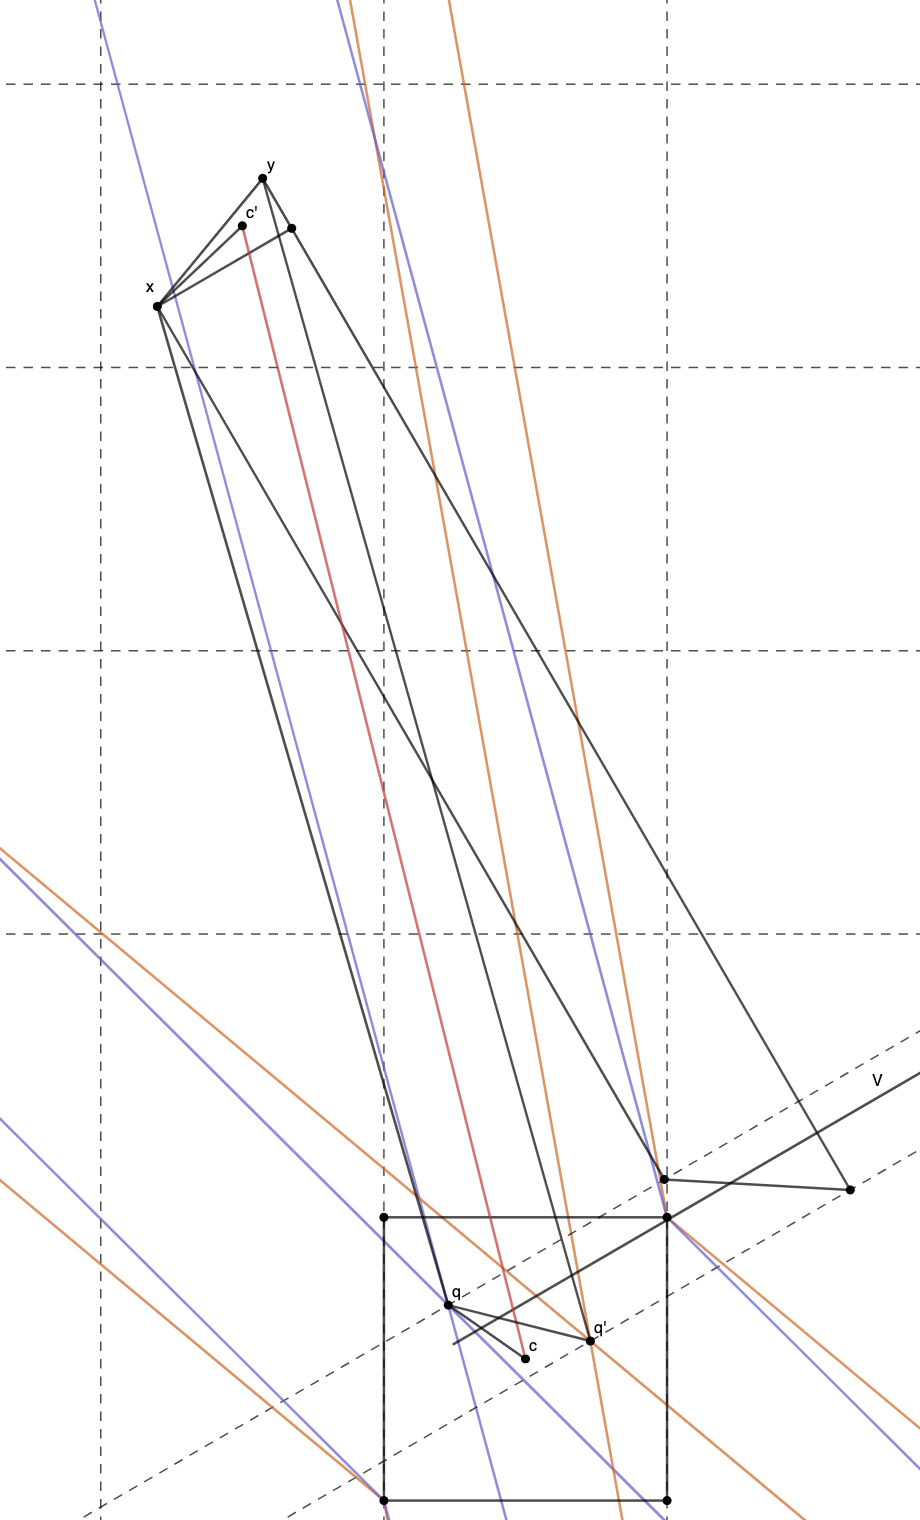
\includegraphics[width=.66\textwidth]{images/guaranteeContainalpha12.png}
    \caption{An example of containment in the proof on $\rr^2$}
\end{figure}




\newpage
\subsection{June 22 Doubling Measure for Cubes and other Lemmas}

\begin{lemma}\label{lemma:ofthmA} 
    Let $\mu$ be a pointwise doubling measure on $\rr^n$. For $\mu$-a.e. $x \in \rr^n$, $Q$ with side length $2^{-|k|}$ containing $x$, there is an $m$-plane $V$ and an $\alpha \in(0,1)$ such that with a scaling constant $s$,
    \begin{equation}\label{eq:lemmaofthmAeq}
        \lim_{|k| \rightarrow \infty} \frac{\mu\left(C_\calB(Q, V, \alpha)\right)}{\mu(sQ))}=0
    \end{equation}
    if and only if $\mu$ is carried by Lipschitz graphs.
\end{lemma}
\textit{Proof for Sufficient Condition.} With the same notation in Lemma \ref{lemma:CBQ2carried}, where $E = \bigcup_{i=1}^\infty E_i$ and for $\mu$-a.e. $y\in E$, $E_i = Q_{E_i}\cap E$. Fix a $Q_{E_i}$, by (\ref{eq:lemmaofthmAeq}), for any $\epsilon>0$, there exists $N_i\in\nn$ such that when $k\geq N_i$, 
$$\left |\frac{\mu\left(C_\calB^2(Q_{E_i}, V, \alpha)\right)}{\mu(sQ_{E_i}))}\right | < \epsilon$$
Define $r = 2^{-|k|}s$, then $\lim_{|k|\rightarrow\infty} r = 0$. Thus, there exists $N^\prime\in \nn$ such that whenever $k\geq N^\prime$, $|r|<\epsilon$. Thus, choosing $N=\max\{\{N_i\}\cup\{N^\prime\}$, two inequalities hold for every $Q_{E_i}$ in the meanwhile. Then for $\mu$-a.e. $y\in Q_{E_i}$ and by (\ref{eq:CysubsetCQ}), $s\cdot Q_{E_i}\subset B(y, r)$ and $C_\calB(y, r, V, \alpha)\subset C_\calB(y, V, \alpha)\subset C_\calB^2(Q_{E_i}, V, \alpha)$. Thus, let $\delta = \epsilon$, we have for any $\epsilon>0$ there exists $\delta>0$ such that whenever $|r-0|<\delta$, by containment, 
\begin{equation}
    \left|  \frac{\mu(C_\calB(y, r, V, \alpha))}{\mu(B(y, r))} \right| \leq \left |\frac{\mu\left(C_\calB^2(Q_{E_i}, V, \alpha)\right)}{\mu(sQ_{E_i}))}\right| < \epsilon
\end{equation}
Therefore
\begin{equation}\label{eq:lemmathmAeq2}
    \lim_{r\downarrow 0} \frac{\mu(C_\calB(y, r, V, \alpha))}{\mu(B(y, r))} = 0
\end{equation}
Applying \ref{thm:NaplesthmD}, the conclusion holds.


\begin{customthm}{{\cite[Theorem D]{naples2020}}}\label{thm:NaplesthmD}
    Let $\mu$ be a pointwise doubling measure on a separable, finite or infinite dimensional Hilbert space $H$. For $\mu$-a.e. $x \in H$ there is an $m$ -plane $V$ and an $\alpha \in(0,1)$ such that
$$
\lim _{r \downarrow 0} \frac{\mu\left(C_{\mathcal{B}}(x, r, V, \alpha)\right)}{\mu(B(x, r))}=0
$$
if and only if $\mu$ is carried by Lipschitz graphs.
\end{customthm}




\begin{lemma}
    If $\mu$-a.e. $x\in \rr^n, \mu(B(x, 2r))\leq K\mu(B(x,r)), K\in\zz^+$, then
    $\mu(2Q)\leq K^3 \mu(Q)$ where $Q$ is the dyadic cube, 2$Q$ is the cube with double dilation of $Q$. 
\end{lemma}
\begin{proof} By the half open definition of the dyatic cube, for $\mu$-a.e. $x\in \rr^n$, $x$ must in only one cube, named $Q$ with $\side Q = 2^{-|k|}$. Let $r = \frac{1}{2}\side Q$, then by the containment
    \begin{equation}
        \mu(4Q)\leq \mu(B(x, 8r))\leq K^3 \mu(B(x, r)) \leq K^3 \mu(2Q)
    \end{equation}

    \begin{equation}
        \mu(5Q) \leq \mu(B(x, 16r)) \leq K^4\mu(B(x,r))\leq K^4\mu(3Q)
    \end{equation}
\end{proof}
There always exists $k$ such that any $\mu$-a.e. $x$ must in $1/2 Q$ with side length $2^{-|k|}$. Then similarly we have $\mu(2Q)\leq K^3\mu(Q)$.

\begin{figure}[H]
    \centering
    \includegraphics[width=.66\textwidth]{images/doubleMucube.png}
    \caption{An example of containment in the proof on $\rr^2$}
\end{figure}

\newpage
\subsection{June 21 \texorpdfstring{$\lim_{Q\rightarrow x}\mu(C_\calB(Q, V, \alpha))/\mu(sQ) = 0$}{Lg}}

\begin{definition}[Alternative Definition for Bad Cones at a Cube] For the dyadic cube $Q$, let $R$ denote the dyadic cube with the same side length as $Q$ in the cube system. Then definitions of bad cones at a cube can be 
    \begin{equation*}
        C_\calB^{k,1}(Q, V, \alpha) = \{R: R\cap C_\calB^k(Q, V, \alpha) \neq \emptyset\}, \quad
        C_\calB^{k,2}(Q, V, \alpha) = \{R: R\subset C_\calB^k(Q, V, \alpha)\} 
    \end{equation*}
for $k=1,2$.
\end{definition}




\begin{customthm}{A}\label{thmA} 
    Let $\mu$ be a pointwise doubling measure on $\rr^n$. For $\mu$-a.e. $x \in \rr^n$, $Q$ that contains $x$, there is an $m$-plane $V$ and an $\alpha \in(0,1)$ such that with a scaling constant $s$,
    \begin{equation}\label{thmAeq}
        \lim_{Q \downarrow x} \frac{\mu\left(C_\calB(Q, V, \alpha)\right)}{\mu(sQ))}=0
    \end{equation}
    if and only if $\mu$ is carried by Lipschitz graphs.
\end{customthm}
\textit{Proof for Sufficient Condition.} With the same notation in Lemma \ref{lemma:CBQ2carried}, where $E = \bigcup_{i=1}^\infty E_i$ and for some $y_i\in E$, $E_i=\{y_i\}\subset Q_{E_i}$. Fix $y_0\in Q_{E_i}$ and by (\ref{eq:CysubsetCQ}), when $|k|\downarrow 0$, $C_\calB(y_0, V, \alpha)\subset C_\calB^2(Q_{E_i}, V, \alpha)$. Then if $r=s\cdot 2^{-|k|}$, we have $s\cdot Q_{E_i}\subset B(y_0, r)$ and $C_\calB(y_0, r, V, \alpha)\subset C_\calB(y_0, V, \alpha)\subset C_\calB^2(Q_{E_i}, V, \alpha)$. Now as $|k|\downarrow 0\Rightarrow r\downarrow 0$ and by (\ref{thmAeq}),
\begin{equation}\label{eq:thmAeq1}
    \lim_{r\downarrow 0} \frac{\mu(C_\calB(y_i, r, V, \alpha))}{\mu(B(y_i, r))} \leq \lim_{Q \downarrow x} \frac{\mu\left(C_\calB(Q, V, \alpha)\right)}{\mu(sQ))}=0
\end{equation} 
Applying \ref{eq:thmAeq1} for every $y$ in every $Q_{E_i}$, and \ref{thm:NaplesthmD}, the conclusion holds.




\newpage
\subsection{June 17-20 \texorpdfstring{$\mu(C_\mathcal{B}^2(Q, V, \alpha)) = 0 \Rightarrow \mu$ Carried by Lipschitz Graphs}{Lg}}

\begin{lemma}\label{lemma:CBQ2carried}
    Let $\mu$ be a Radon measure on $\rr^n$, $V$ be an $m$-dimensional linear plane in $\rr^n$, $\alpha\in(0,1)$. Suppose $E\subset \rr^n$ such that for $\mu$-a.e. $y\in E$, and for every dyadic cube $Q$ containing $y$, 
    \begin{equation}\label{muB2=0}
        \mu(C_\calB^2(Q, V, \alpha)) = 0
    \end{equation}
    Then $\mu$ is carried by $m$-Lipschitz graphs(i.e. $E$ is contained $\mu$-a.e. in an m-Lipschitz graph.)
\end{lemma}

\begin{proof}
    we first claim that if every dyadic cube $Q\ni y$ in the form of (\ref{eq:dyadiccube}) with side length $2^{-|k|}$ satisfies (\ref{muB2=0}), 
    then
    \begin{equation}\label{muBx=0}
        \mu(C_\calB(y, V, \alpha)) = 0
    \end{equation}
    Note that each $y\in E$ is contained in no more than one half open $Q$. Let $Q_{E_i}$ denote the dyadic cube that contains $E_i\subset E$ such that $E_i$ consists of all $y\in E\cap Q_{E_i}$ and $E$ is the countable union of disjoint $E_i$. For any two points $x_1\in Q_{E_i}, y_1\in E_i$, we have $|x_1-y_1|\leq \sqrt{n}\cdot 2^{-|k|}$. Consider that if any $p\in C_\calB(y_1, V, \alpha)$, we have $\dist(p-y_1, V) > \alpha|p-y_1|$ by definition of bad cones. Now let $\epsilon>0$ such that $\dist(p-y_1, V) \geq \alpha (|p-y_1|+\epsilon)$. When $|k|\rightarrow \infty, 2^{-|k|}\rightarrow 0$, so there exists $N\in\nn$ such that whenever $|k|\geq N$, for $x_1, y_1\in Q_{E_i}$ we have $|x_1-y_1|<\alpha\epsilon/2<\epsilon/2$, recalling that $\alpha\in(0,1)$. Then
\begin{equation*}
    \begin{aligned} 
        \dist\left(p-x_1, V\right) & \geq \dist(p-y_1, V)-\left|x_1-y_1\right| \\ 
        & \geq \alpha(|p-y_1|+\epsilon)-\alpha(\epsilon / 2) \\ 
        & =\alpha(|p-y_1|+\epsilon / 2) \\ 
        & >\alpha\left(|p-y_1|+\left|x_1-y_1\right|\right) \\ 
        & \geq \alpha\left(\left|p-x_1\right|\right) 
\end{aligned}
\end{equation*}
It follows that $p\in C_{\calB}(x_1, V, \alpha)$, and as $x_1$ is arbitrary point in $Q_{E_i}$, $p\in C_\calB^2(Q_{E_i}, V, \alpha)$. Thus, when $|k|\rightarrow \infty$
\begin{equation}\label{eq:CysubsetCQ}
    C_{\calB}(y_1, V, \alpha)\subset C_\calB(Q_{E_i}, V, \alpha),\quad \forall y_1\in E_i \subset Q_{E_i}
\end{equation}
Then applying (\ref{muB2=0}), 
\begin{equation*}
    \begin{split}
        \mu(\bigcup_{y\in E}C_\calB(y, V, \alpha))
        = \lim_{|k|\rightarrow \infty}\mu\left( \bigcup_{E_i\in E}\bigcup_{y\in Q_{E_i}} C_\calB(y, V, \alpha) \right)  
        \leq \lim_{|k|\rightarrow\infty}\mu\left( \bigcup_{E_i\in E} C_\calB^2(Q_{E_i}, V, \alpha) \right)
        = 0
    \end{split}
\end{equation*}
Therefore, we have (\ref{muBx=0}) for each $y\in E$. Then applying corollary \ref{LisaCoro7.1}, we obtain the desired result. 
\end{proof}



An example of this proof illustrated in $\rr^2$ is shwon in Figure \ref{fig:CB1=CB2}.

\begin{figure}[H]
    \centering
    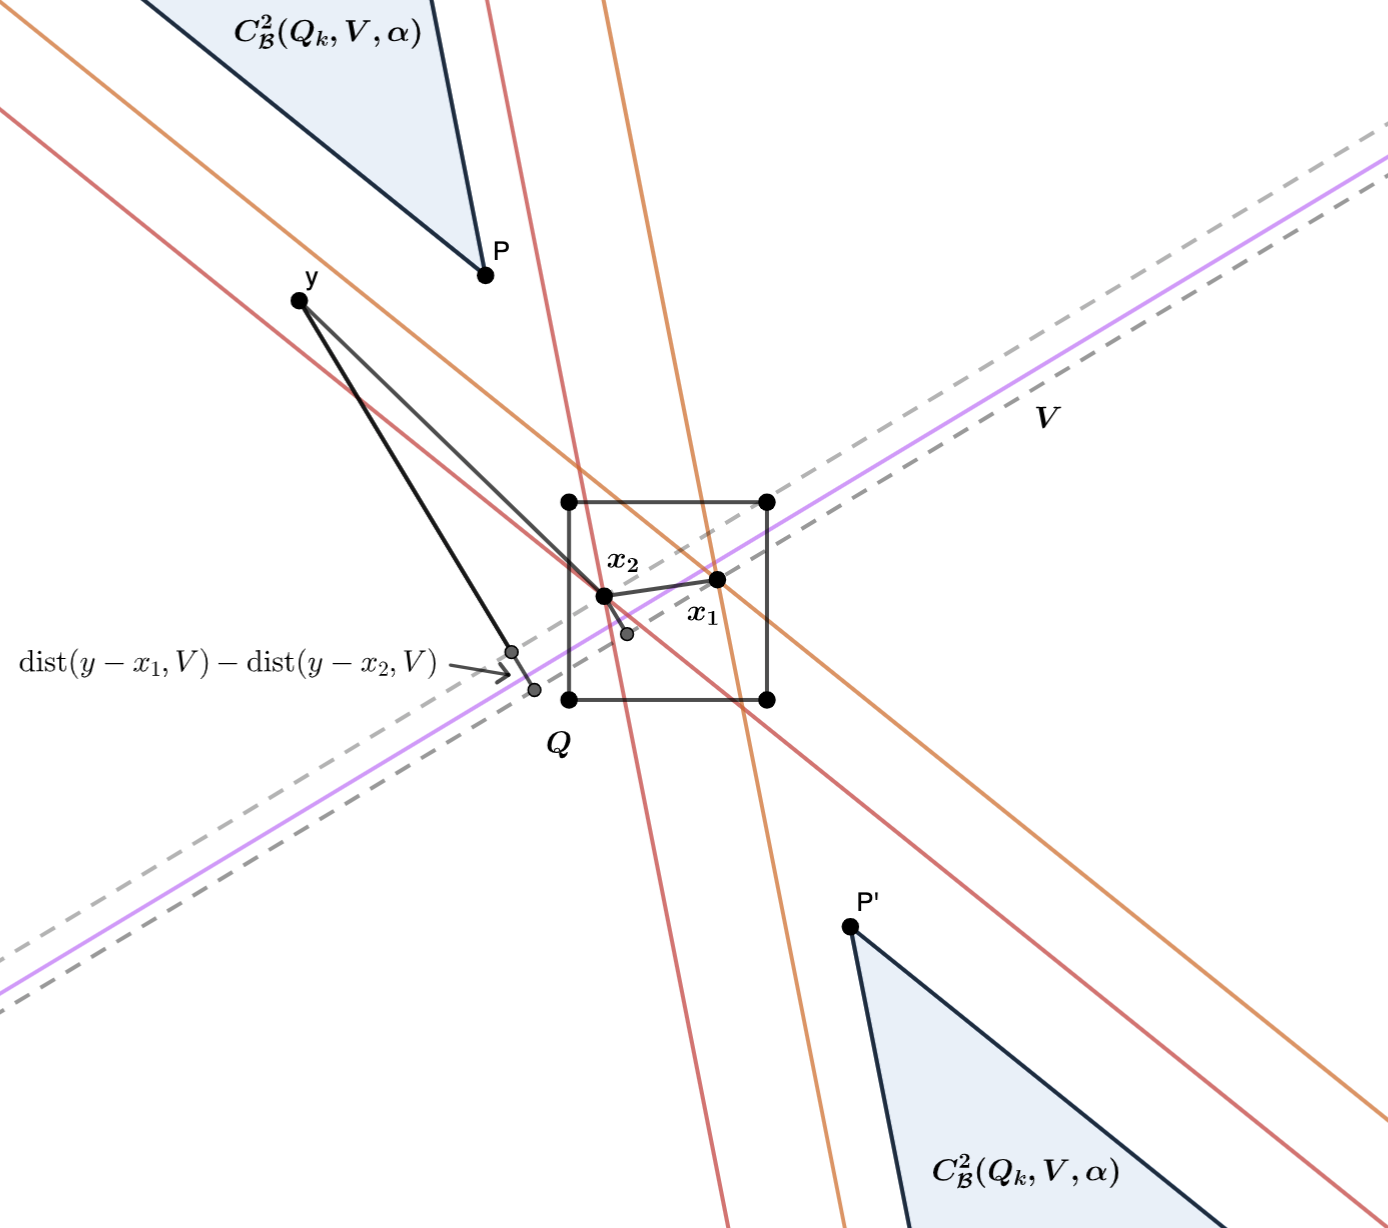
\includegraphics[width=.6\textwidth]{images/CB1=CB2.png}
    \caption{Example visulization of proof in $\rr^2$}
    \label{fig:CB1=CB2}
\end{figure}


\begin{corollary}[{\cite[Corollary 7.1]{naples2020}}]\label{LisaCoro7.1}
    Let $\mu$ be a Radon measure on $H, V$ be an $m$-dimensional linear plane in $H$, $\alpha \in(0,1)$, and $0<r<\infty$. If for $\mu$ -a.e. $x \in H$
   $$
   \mu\left(C_{\mathcal{B}}(x, r, V, \alpha)\right)=0
   $$
   then $\mu$ is carried by $m$-Lipschitz graphs.
\end{corollary}




\newpage
\subsection{June 16 New Cone Definition for Dyadic Cubes}
\begin{definition}[Dyadic Cubes] A dyadic cube $Q$ is a set of the form
    \begin{equation}\label{eq:dyadiccube}
        Q=\left[\frac{j_{1}}{2^{k}}, \frac{j_{1}+1}{2^{k}}\right) \times \cdots \times\left[\frac{j_{n}}{2^{k}}, \frac{j_{n}+1}{2^{k}}\right), \quad k, j_{1}, \ldots, j_{n} \in \mathbb{Z}
    \end{equation}
\end{definition}

\begin{definition}[Bad Cone at a Cube(definition 1)] Let $Q$ be the dyadic cube, then we can have the first definition of bad cone at $Q$ with respect to $V$ and $\alpha$ by:
    $$C^1_{\mathcal{B}}(Q, V, \alpha) := \bigcup_{x\in Q} C_\mathcal{B}(x, V, \alpha), \quad C^1_{\mathcal{B}}(Q, r, V, \alpha) = C^1_{\mathcal{B}}(Q, V, \alpha) \cap B(x,r)$$
    where $V$ is a m-dimensional linear plane through the origin. 
\end{definition}

\begin{definition}[Bad Cone for Cube(definition 2)]
    We can have the second definition of bad cone at $Q$ with respect to $V$ and $\alpha$ with the similar notation:
    $$C^2_{\mathcal{B}}(Q, V, \alpha) := \bigcap_{x\in Q} C_\mathcal{B}(x, V, \alpha), \quad
    C^2_{\mathcal{B}}(Q, r, V, \alpha) = C^2_{\mathcal{B}}(Q, V, \alpha) \cap B(x,r)
    $$
\end{definition}
\begin{figure}[H]
    \centering
    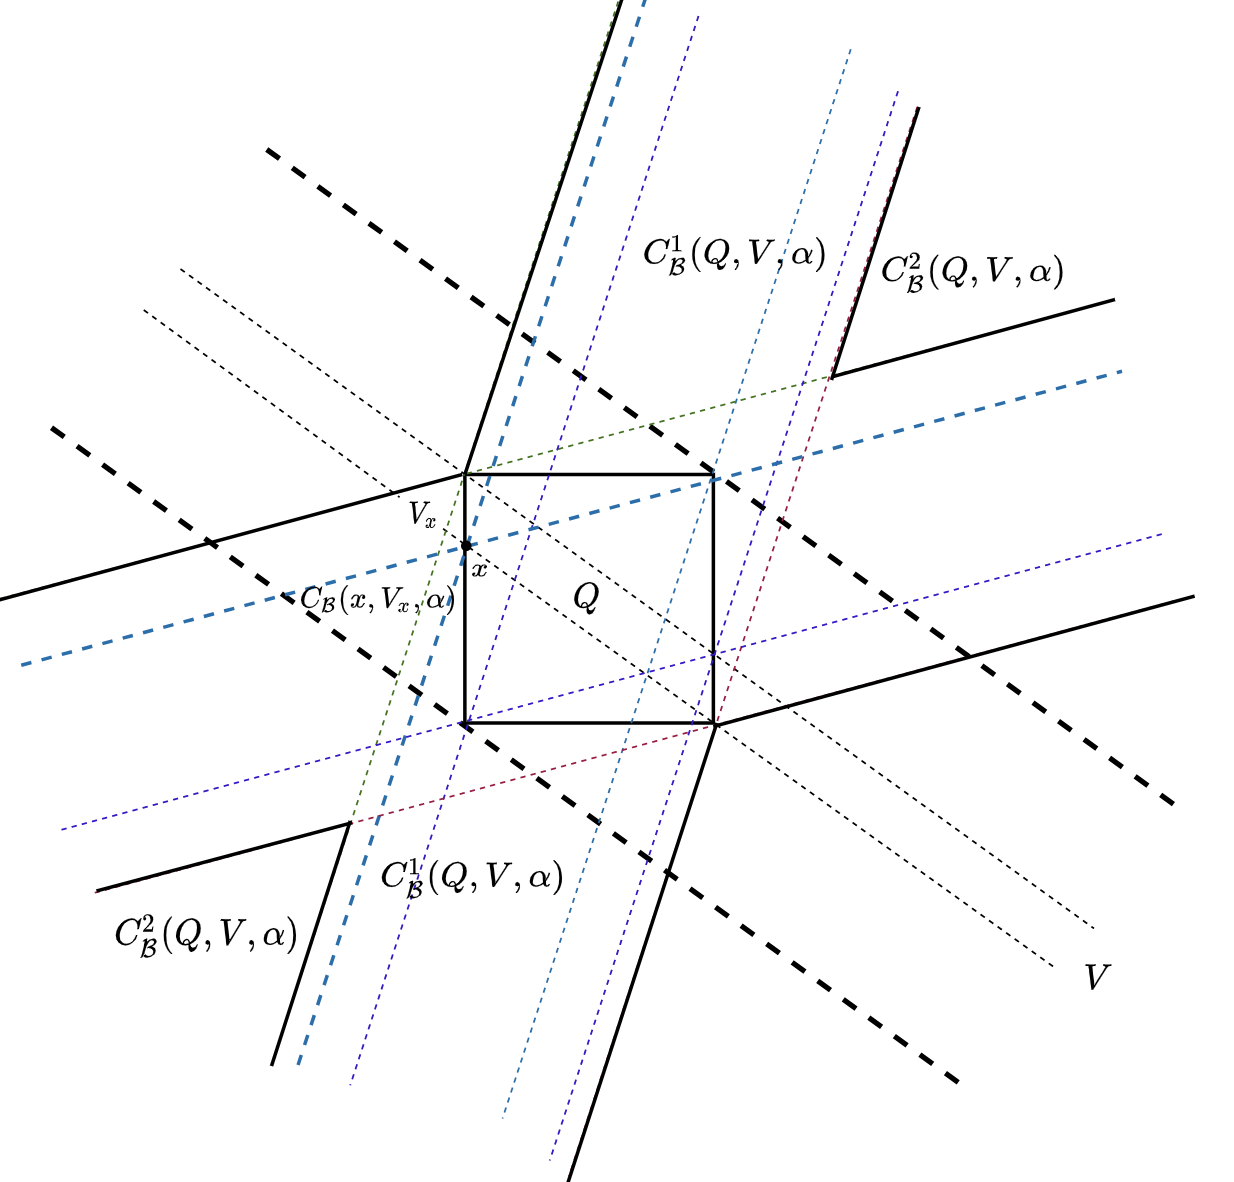
\includegraphics[width=.66\textwidth]{images/cubebadconeDef.png}
    \caption{Visulize two definitions of bad cone at a cube in $\rr^2$}
\end{figure}

\begin{problem}
    Suppose that at $\mu$-a.e. $x$, $\alpha\in(0, 1)$, for all $k$, for every cube $Q\ni x$ of side length $2^{-k}$ satisfies
    $$
    \mu(C^2_\mathcal{B}(Q, V, \alpha)) = 0
    $$ 
    is $\mu$-carried Lipschitz by Lipschitz graphs?
\end{problem}

\newpage
\subsection{June 15 A Proposition of Doubling Measure for Cubes}

\begin{proposition}
    If $\forall x\in \rr^2, \mu(B(x, 2r))\leq K\mu(B(x,r)), K\in\zz^+$, then $\exists R\in \zz^+$ s.t. $\mu(3Q)\leq R\mu(Q)$ where $Q$ is the cube, 3$Q$ is the cube with triple side length with same center as $Q$. 
\end{proposition}
\proof  $\mu(3Q) \leq \mu(B(x, 4\side Q)) \leq K^3\mu(B(x, \frac{1}{2} \side r))\leq K^3 \mu(Q)$ due to doubling measure and containment. 

\begin{figure}[H]
    \centering
    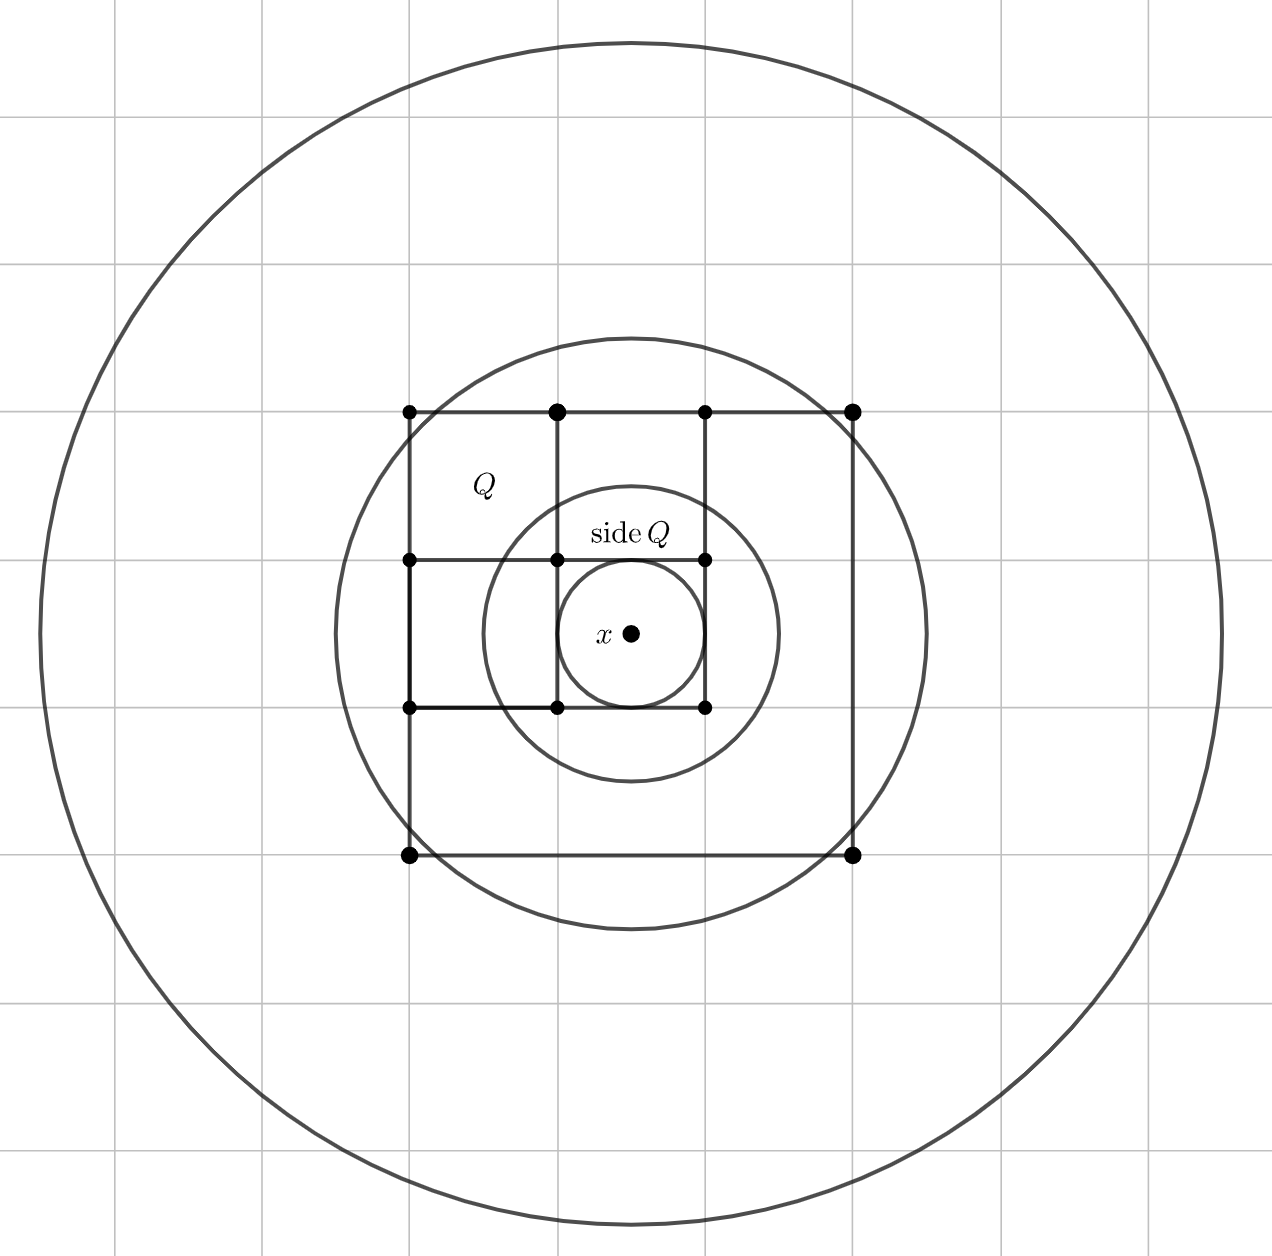
\includegraphics[width=.66\textwidth]{images/tripleMcube.png}
\end{figure}


\newpage
\subsection{June 14 Paper \texorpdfstring{\cite{naples2020}}{Lg} Sec. 7 Graph Rectifiable Measures}

\begin{definition}[Good Cone]
    Let $V$ be a m-dimensional plane in Hilbert space $H$, then we can define the good cone at $x$ with respect to $V$ and $\alpha$ by:
    $$
    C_\mathcal{G}(x, V, \alpha) := \{y\in H: \dist(y-x, V) \leq \alpha |x-y|\}
    $$
    another notation:
    $$
    C_\mathcal{G}(x, r, V, \alpha) = C_\mathcal{G}(x, V, \alpha) \cap B(x, r)
    $$
\end{definition}
\begin{definition}[Bad Cone]
    The bad cone at x with respect to V and $\alpha$:
    $$
    C_\mathcal{B}(x, V, \alpha) := H\setminus C_{\mathcal{G}(x, V, \alpha)}, \quad C_\mathcal{B}(x, r, V, \alpha) = C_\mathcal{B}(x, V, \alpha) \cap B(x, r)
    $$
\end{definition}


\begin{figure}[H]
    \centering
    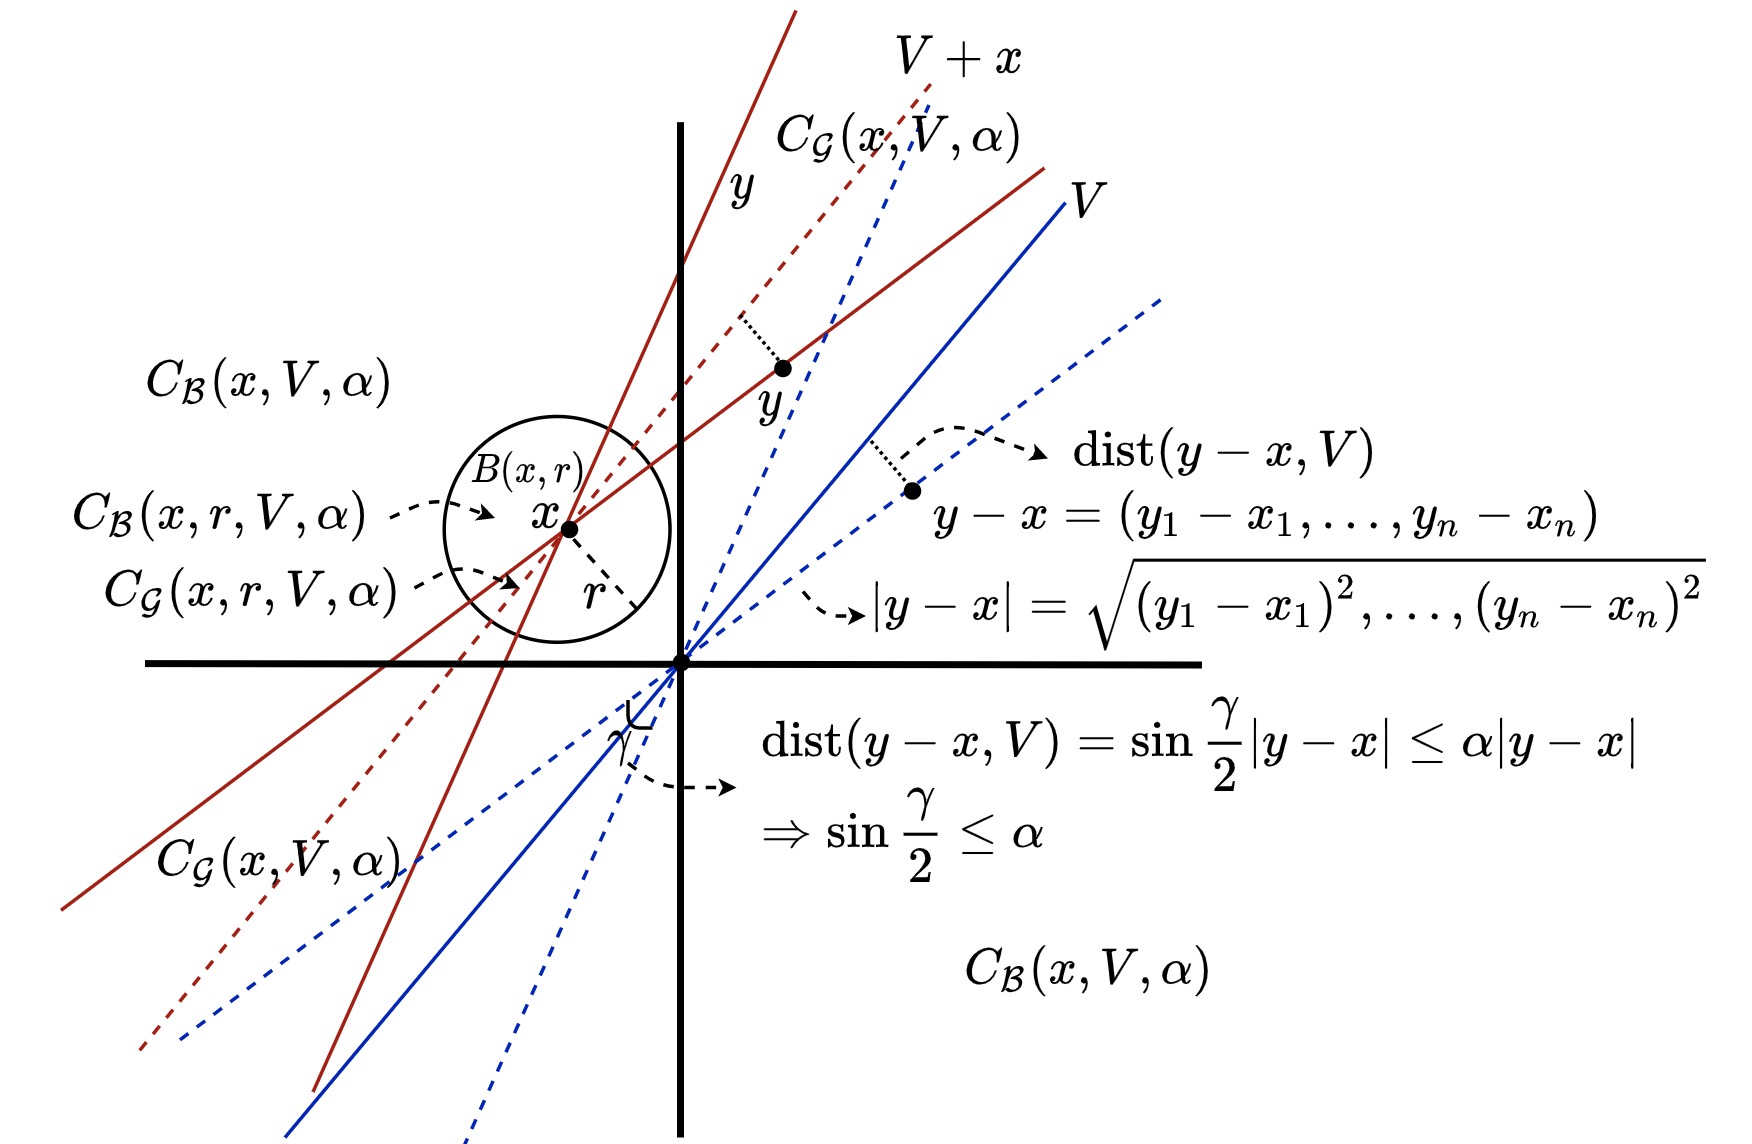
\includegraphics[width=.8\textwidth]{images/conedef.png}
    \caption{Example visualization of definitions related to cones in $\rr^2$}
\end{figure}

\begin{definition}[Carried $\&$ Singular]
   Let $(\mathbb{X}, \mathcal{M})$ be a measurable space, and let $\mathcal{N} \subset \mathcal{M}$ be a family of measurable sets. We say
   \begin{enumerate}[(1)]
       \item $\mu$ is carried by $\mathcal{N}$ if there exist countably many $N_{i} \in \mathcal{N}$ such that $\mu\left(\mathbb{X} \backslash \bigcup_{i} N_{i}\right)=0$;
       \item $\mu$ is singular to $\mathcal{N}$ if $\mu(N)=0$ for every $N \in \mathcal{N}$.    
   \end{enumerate}
   A $\sigma$ -finite measure $\mu$ on $(\mathbb{X}, \mathcal{M})$ can be decomposed uniquely as
       $$
       \mu=\mu_{\mathcal{N}}+\mu_{\mathcal{N}}^{\perp}
       $$
       where $\mu_{\mathcal{N}}$ is carried by $\mathcal{N}$ and $\mu_{\mathcal{N}}^{\perp}$ is singular to $\mathcal{N}$. 
\end{definition}

\begin{theorem}[Theorem 7.1 Geometric Lemma] $ $\\
    Let $F \subset H$, let $V$ be an $m$-dimensional linear plane in $H$, and let $\alpha \in(0,1) .$ If
$$
F \backslash C_{\mathcal{G}}(x, V, \alpha)=\emptyset \text { for all } x \in F
$$
then $F$ is contained in an $m$ -Lipschitz graphs. In particular, $F \subset \Gamma$ where $\Gamma$ is a Lipschitz graph with respect to $V$ and the Lipschitz constant corresponding to $\Gamma$ is at most $1+1 /\left(1-\alpha^{2}\right)^{1 / 2} .$
\end{theorem}
\proof Let $x \in F$. Let $P_{V}: H \rightarrow V$ denote standard projection onto the $m$ -plane $V$. Suppose that $\left|P_{V} x-P_{V} y\right|<\left(1-\alpha^{2}\right)^{1 / 2}|x-y|$. Then $y \in C_{\mathcal{B}}(x, V, \alpha)$, and by assumption of $F$ this means that $y \notin F$. Thus we may assume that if $x, y \in F$ then
$$
\left|P_{V} x-P_{V} y\right| \geq\left(1-\alpha^{2}\right)^{1 / 2}|x-y|
$$
From this inequality we see that $P_{V} \mid F$ is one-to-one with Lipschitz inverse $f=\left(P_{V} \mid F\right)^{-1}$ and $\operatorname{Lip}(f) \leq\left(1-\alpha^{2}\right)^{-1 / 2}$. Note that $F=f\left(P_{V} \mid F\right)$. Then there exists a Lipschitz extension $\tilde{f}: V \rightarrow$ $H$ so that $F \subset \tilde{f}(V)$. Thus the desired result holds. 

\begin{corollary}[Corollary 7.1]
 Let $\mu$ be a Radon measure on $H, V$ be an $m$-dimensional linear plane in $H$, $\alpha \in(0,1)$, and $0<r<\infty$. If for $\mu$ -a.e. $x \in H$
$$
\mu\left(C_{\mathcal{B}}(x, r, V, \alpha)\right)=0
$$
then $\mu$ is carried by $m$ -Lipschitz graphs.
\end{corollary}
\proof Let $F$ denote the set of $x \in H$ that satisfy (18). We may assume $F \subset B(0, r / 2)$; otherwise we may write $F$ as a union of countably many sufficiently small sets and show that each one is $m$ -graph rectifiable. Let $\left\{x_{i}\right\}$ be a countable dense subset of $F .$ It follows from (18) and the containment $F \subset B(0, r / 2)$ that for each $x_{i}$ there exists $F_{i} \subset F$ such that
$$
F_{i} \cap C_{\mathcal{B}}\left(x_{i}, r, V, \alpha\right)=F_{i} \cap C_{\mathcal{B}}\left(x_{i}, V, \alpha\right)=\emptyset
$$
and $\mu\left(F \backslash F_{i}\right)=0$. Define $F^{\prime}:=\bigcap_{i=1}^{\infty} F_{i}$. Then
$$
\mu\left(F \backslash F^{\prime}\right)=\mu\left(F \backslash \bigcap_{i=1}^{\infty} F_{i}\right)=\mu\left(\bigcup_{i=1}^{\infty} F \backslash F_{i}\right) \leq \sum_{i=1}^{\infty} \mu\left(F \backslash F_{i}\right)=0
$$
We claim that $F^{\prime} \cap C_{\mathcal{B}}(x, V, \alpha)=\emptyset$ for every $x \in F^{\prime} .$ Fix $x \in F^{\prime}$, and let $y \in C_{\mathcal{B}}(x, V, \alpha)$.
By definition of bad cone we have that $\dist(y-x, V)>\alpha|y-x|$. Now let $\epsilon>0$ such that $\dist(y-x, V) \geq \alpha(|y-x|+\epsilon)$. Recalling that $0<\alpha<1$, choose $x_{i}$ such that $\left|x_{i}-x\right|<\alpha \epsilon / 2<$
$\epsilon / 2 .$ Then
$$
\begin{aligned}
\dist\left(y-x_{i}, V\right) & \geq \dist(y-x, V)-\left|x-x_{i}\right| \\
& \geq \alpha(|y-x|+\epsilon)-\alpha(\epsilon / 2) \\
&=\alpha(|y-x|+\epsilon / 2) \\
&>\alpha\left(|y-x|+\left|x_{i}-x\right|\right) \\
& \geq \alpha\left(\left|y-x_{i}\right|\right) .
\end{aligned}
$$
In particular, we conclude that $y \in C_{\mathcal{B}}\left(x_{i}, V, \alpha\right) .$ Since $F_{i} \cap C_{\mathcal{B}}\left(x_{i}, V, \alpha\right)=\emptyset$, it must be that case that $y \notin F_{i}$. It follows that $y \notin F^{\prime}$, and thus $F^{\prime} \cap C_{\mathcal{B}}(x, V, \alpha)=\emptyset$ for all $x \in F^{\prime}$. By an application of Theorem $7.1$ we conclude that there exists an $m$ -Lipschitz graph $\Gamma$ such that $F^{\prime} \subset \Gamma$, so $\mu(F \backslash \Gamma)=0$.

\begin{lemma}[Lemma 7.2]
    Let $\mu$ be a Radon measure on $H$. For $x_{0} \in H, V$ an $m$-dimensional linear plane, $\alpha \in(0,1)$, and parameter $K>0$, let $E$ denote the set of points $x \in H$ such that
(i) The sequence of functions
$$
f_{r}(x):=\frac{\mu\left(C_{\mathcal{B}}(x, r, V, \alpha)\right)}{\mu(B(x, r))}
$$
converges to 0 uniformly on $E$, and
(ii) there exists $r_{1}>0$ such that at every $x \in E$,
$$
\mu(B(x, 2 r)) \leq K \mu(B(x, r)) \text { for all } r \in\left(0, r_{1}\right]
$$
Then $E$ is $\mu$ -carried by $m$ -Lipschitz graphs with Lipschitz constants depending on at most $K$ and $\alpha .$
\end{lemma}
\proof Fix $\delta>0$. By uniform convergence, choose $r_{\delta} \leq r_{1}$ such that for all $r<r_{\delta}$ and for all $x \in E$
(19)
$$
\frac{\mu\left(C_{\mathcal{B}}(x, 2 r, V, \alpha)\right)}{\mu(B(x, 2 r))}<\delta
$$
Fix $x \in E$, and define $S:=E \cap C_{\mathcal{B}}(x, r, V, 2 \alpha)$. Assuming the set is non-empty, fix $y_{0} \in S$ such that $\left|x-y_{0}\right|=\max _{y \in S}|a-y|=: \lambda r$ for some $0<\lambda \leq 1$. As an application of Lemma $7.1$ choose $\eta_{\alpha}$ such that $B\left(y_{0}, \eta_{\alpha} \lambda r\right) \subset C_{\mathcal{B}}(x, 2 r, V, \alpha) .$ Let $d=\log _{2}\left(\frac{\lambda+2}{\eta_{\alpha} \lambda}\right)$. Then
$$
2^{d} \eta_{\alpha} \lambda r=\frac{\lambda+2}{\eta_{\alpha} \lambda} \eta_{\alpha} \lambda r=(\lambda+2) r=\left|x-y_{0}\right| r+2 r .
$$
In particular, for the specified value of $d, B(x, 2 r) \subset B\left(y_{0}, 2^{d} \eta_{\alpha} \lambda r\right) .$ Applying condition (ii) of the set $E$ at the point $y_{0}$ we see that
$(20)$
$\mu\left(C_{\mathcal{B}}(x, 2 r, V, \alpha)\right) \geq \mu\left(B\left(x, \eta_{\alpha} \lambda r\right)\right) \geq K^{-d} \mu\left(B\left(y_{0}, 2^{d} \eta_{\alpha} \lambda r\right)\right) \geq K^{-d} \mu(B(x, 2 r))$
Combining inequalities (19) and (20), we get the density ratio bounds
$$
\delta>\frac{\mu\left(C_{\mathcal{B}}(x, 2 r, V, \alpha)\right)}{\mu(B(x, 2 r))} \geq K^{-d}
$$
for all $r<r_{\delta}$. In particular, this implies that $d>\frac{-\log (\delta)}{\log K}$. Equivalently,
$$
\log \left(\frac{\lambda+2}{\eta_{\alpha} \lambda}\right)>\frac{-\log \delta}{\log K}
$$
so that if $\delta$ is chosen to be less than $2^{-\log K \log \left(\frac{5}{\eta_{\alpha}}\right)}$ then $\lambda<\frac{1}{2}$. From this result we conclude that for $r<r_{\delta}$ and for all $y \in S,|x-y|<\frac{1}{2} r$. Letting $r \downarrow 0$ we conclude that $\mu\left(E \cap C_{\mathcal{B}}\left(x, r_{\delta}, V, 2 \alpha\right)\right)=0$. Thus we can apply Corollary $7.1$, and we obtain the desired conclusion. 

